\subsection{Data Analysis Plan}

\subsubsection{Picarro G2401}

The analyzer that will be used is the model Picarro G2401. It uses near-infrared Cavity Ring Down Spectroscopy (CRDS) technology and is capable of measuring four atmospheric trace gases simultaneously and continuously ($CO, CO_2, CH_4, H_2O$).

The CRDS technique's basic principle is shown in Figure \ref{fig:CRDS}. Light from a semiconductor diode laser is used. There is an optical cavity filled with the gas that has to be analyzed and the aim is to determine the decay time of the diode laser light. As it can be seen in Figure \ref{fig:CRDS}, the sample gas is introduced in a cavity with three high-reflectivity mirrors. When the laser is shut off, the light that was circulating in the cavity decays with a characteristic time which is measured. If the wavelength of the injected light does not match any absorption feature of any gas in the cavity, the decay time is dominated by mirror loss and it is very long. On the other side, when the wavelength of the injected light is resonant with an absorption feature of a species in the cavity, the decay time is short and decreases as the reciprocal of the species concentration.



\begin{figure}[H]
    \begin{align*}
        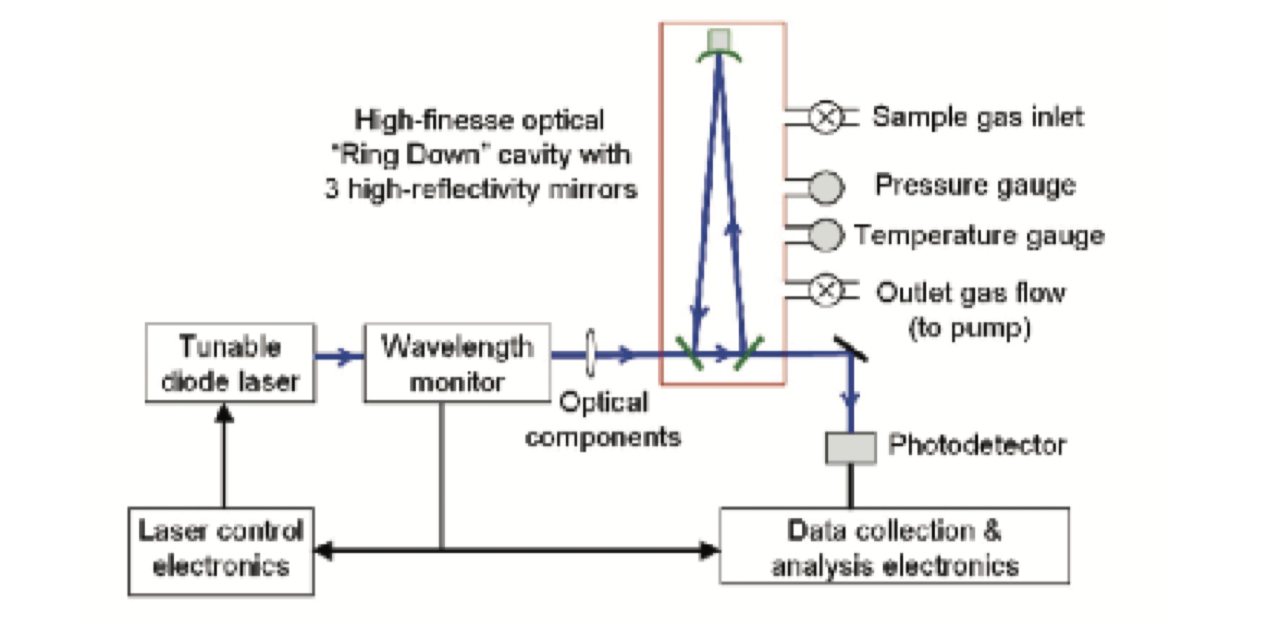
\includegraphics[width=0.9\linewidth]{7-data-analysis-and-results/img/CRDS.png}
    \end{align*}
    \caption{Schematics of CRDS Analyzer Showing Optical Cavity and Sample Gas Flow \cite{Picarro}.\label{fig:CRDS}}
\end{figure}


Figure \ref{fig:Picarro-interfaces} shows the back of the analyzer with gas supply, electrical and computer connections. The analyzer can be configured to deliver data in different formats: digital or analogue. When the main power is turned on the analyzer will automatically start, including the Graphical User Interface (GUI). 

\begin{figure}[H]
    \begin{align*}
        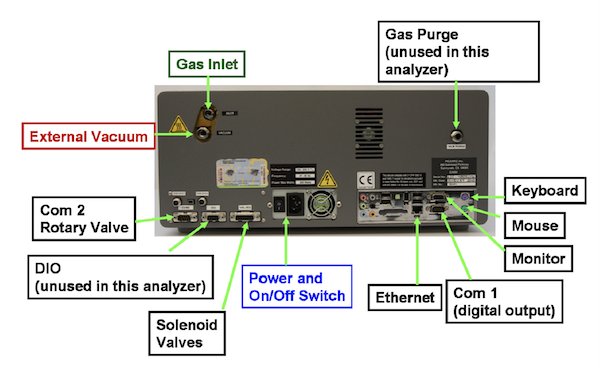
\includegraphics[width=0.9\linewidth]{7-data-analysis-and-results/img/Picarro-interfaces.png}
    \end{align*}
    \caption{Back of Picarro G2401 Analyzer Showing Gas Supply, Electrical and Computer Connections \cite{Picarrouserguide}.\label{fig:Picarro-interfaces}}
\end{figure}


Before the Picarro analyzer is ready for analysis, it is necessary to run a calibrating gas through it in order to remove moisture inside and to have stable measurements to compare with. Figure \ref{fig:picarro-connections} shows the Picarro set up at FMI in Sodankyl\"{a}. A three way valve controls which is the gas flowing into the analyzer. The tube labelled as "AIRCORE" is the one to be connected to the sample, either sampling bags or CAC. The tube labelled as "PICARRO" is the one that goes to the Picarro's inlet and the third tube, without a label, is connected to the calibrating gas bottle.This set up allows easy changing between the samples, dry gas and fill gas with the calibrating gas without getting moisture inside.

\begin{figure}[H]
    \begin{align*}
        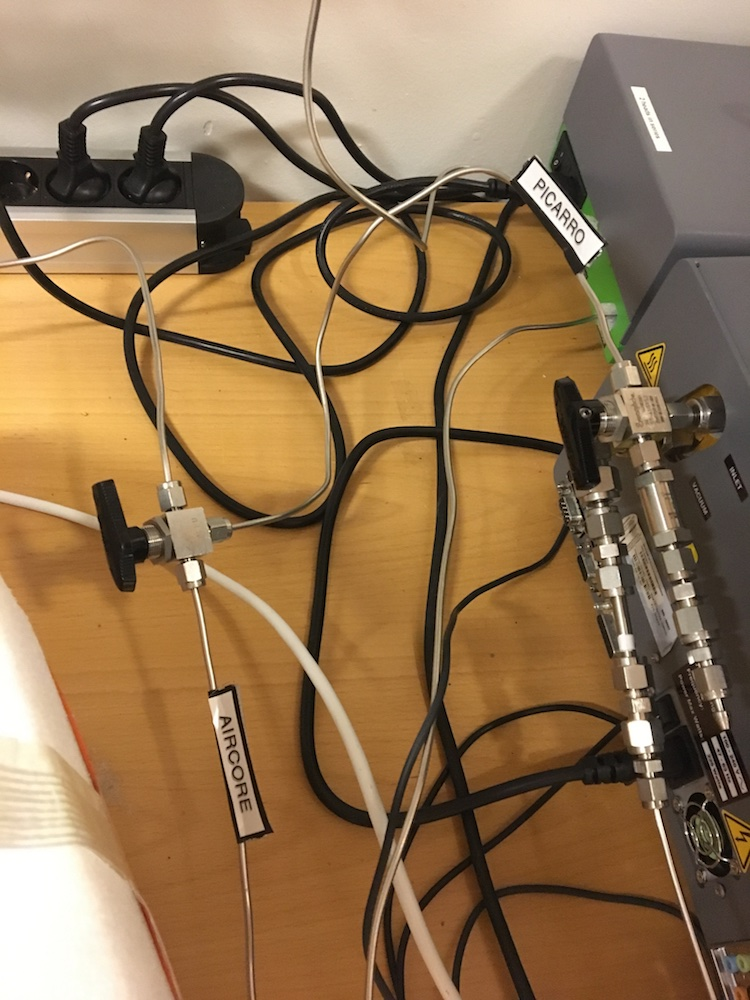
\includegraphics[width=0.9\linewidth]{7-data-analysis-and-results/img/picarro-connections.jpeg}
    \end{align*}
    \caption{Picarro Set-up Connections at FMI in Sodankyl\"{a}. \label{fig:picarro-connections}}
\end{figure}

Figure \ref{fig:picarro-GUI} shows the Picarro GUI during analysis. From top to bottom: $CO_2$ ppm, $CO$ ppm, $CH_4$ ppm and cavity pressure. These options can be changed during analysis as it only means that those are the ones being displayed. Figure \ref{fig:picarro-GUI} was taken minutes after a change between dry gas-sample had been done so a change in the concentrations of $CO_2$ and $CH_4$ can be easily appreciated. 
The Picarro analyzer does not only give information about the displayed parameters, all the data is saved in a .dat file to be analyzed afterwards. The most relevant logged parameters are time, date, ambient pressure, cavity pressure, cavity temperature, $CO$ concentration, $CO_2$, $CH_4$ and $H_2O$ normal and dry concentration. The dry concentration is a correction done automatically by the Picarro analyzer taking into account the moisture inside the analyzer. 

\begin{figure}[H]
    \begin{align*}
        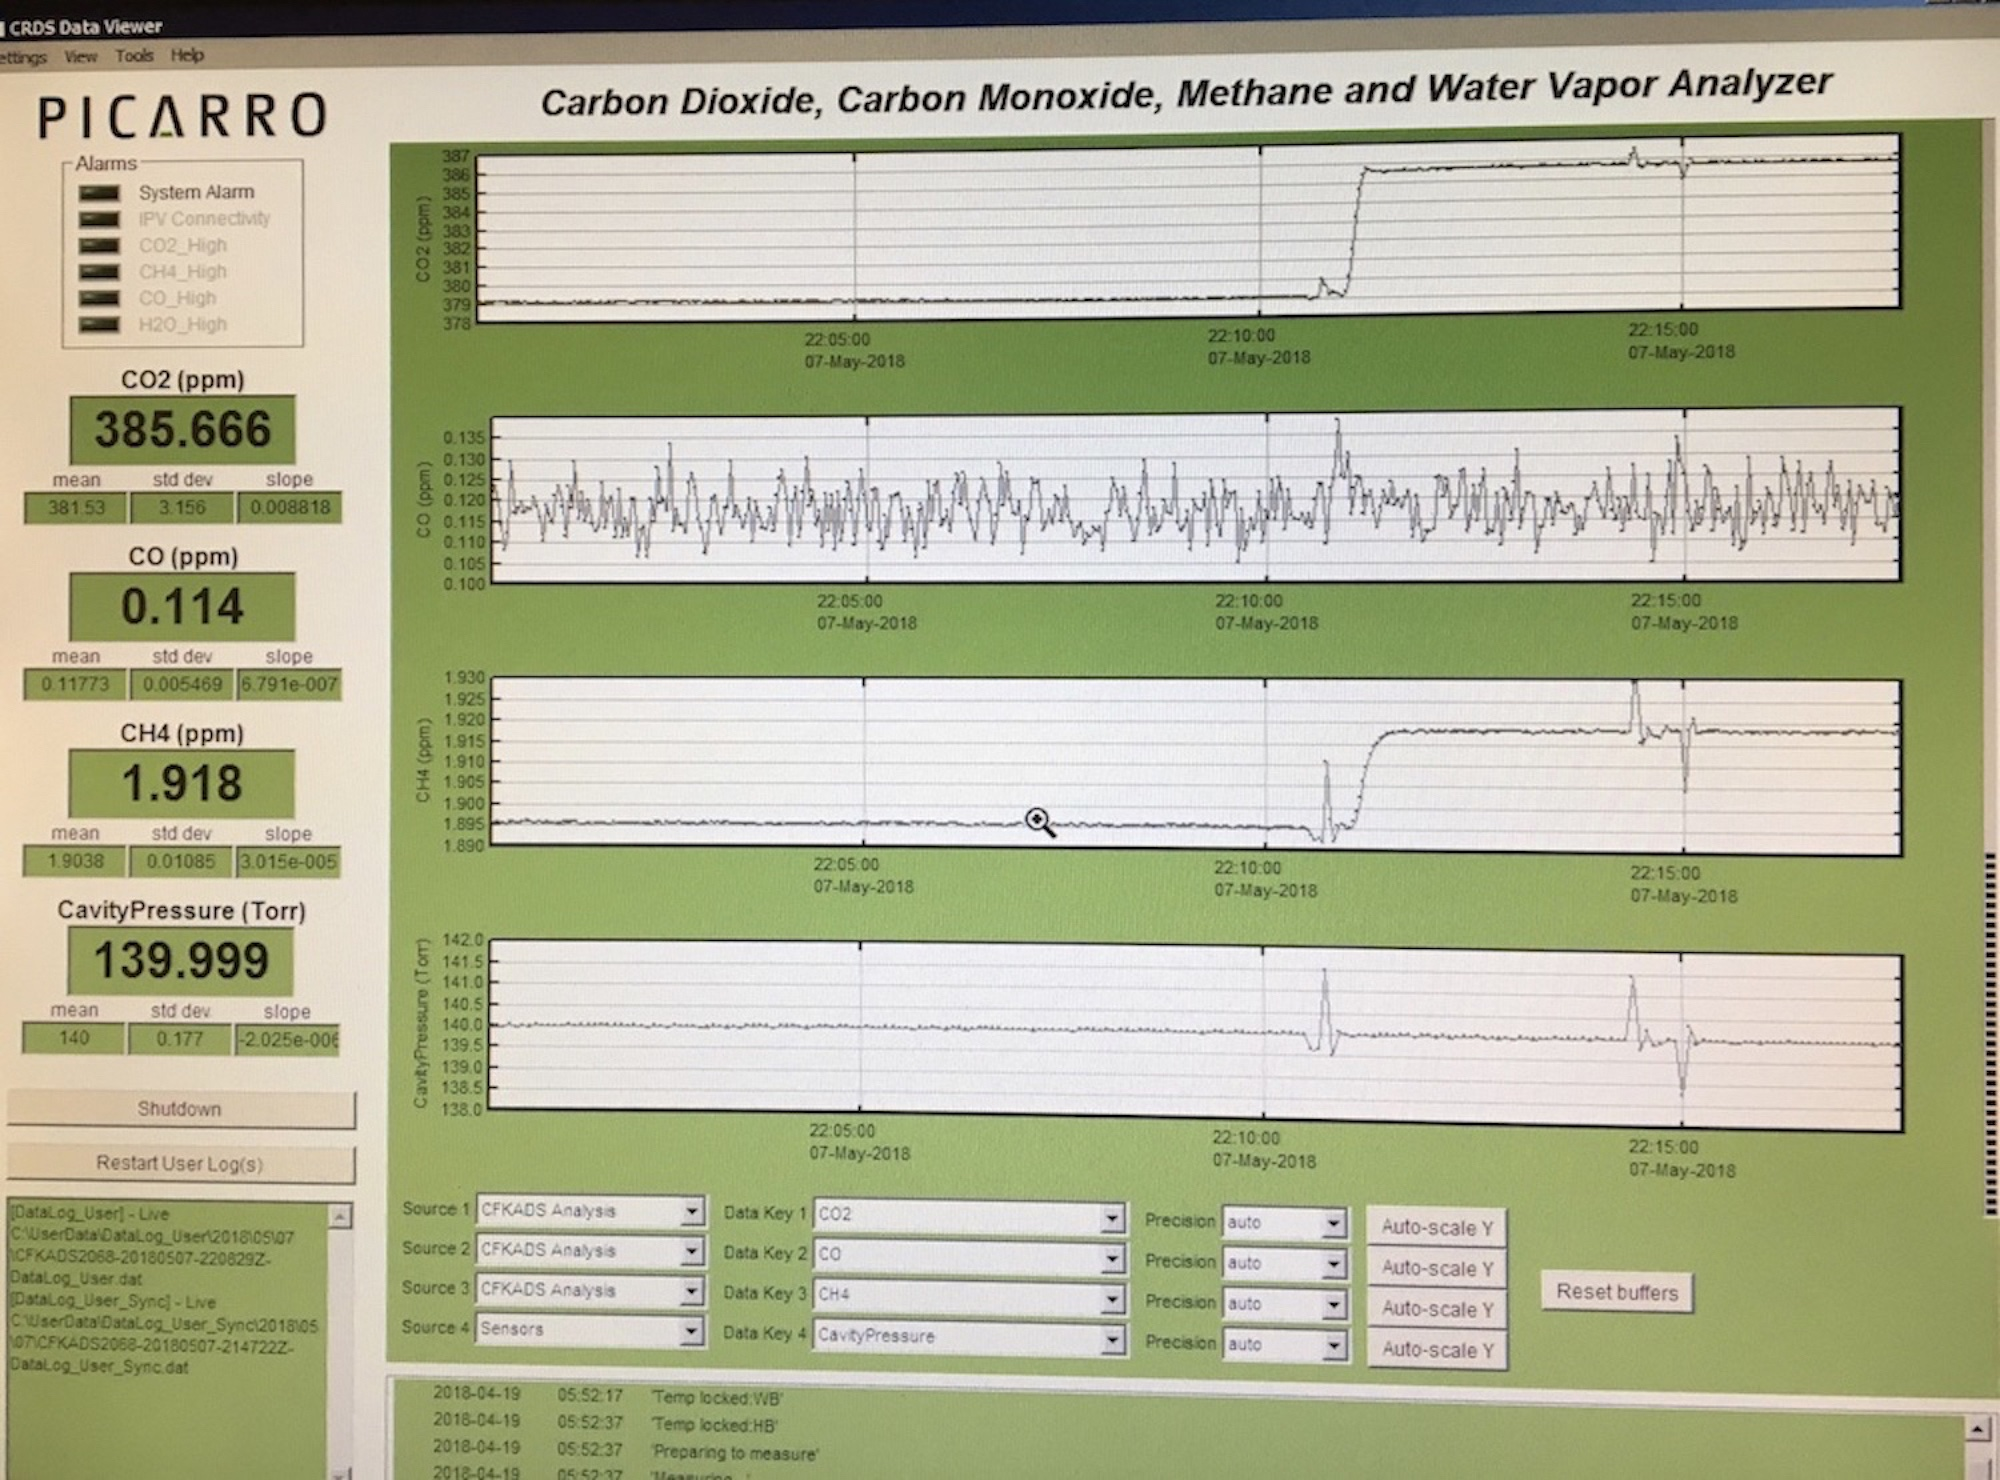
\includegraphics[width=0.9\linewidth]{7-data-analysis-and-results/img/picarro-GUI.jpeg}
    \end{align*}
    \caption{Picarro Graphical User Interface. From Top to Bottom: $CO_2$ ppm, $CO$ ppm, $CH_4$ ppm and Cavity Pressure. \label{fig:picarro-GUI}}
\end{figure}


\subsubsection{Analysis Strategy}

As it has been mentioned in the previous section, during the flight, calibrating gas will be flowing through the Picarro G2401. After the flight, the collected samples from the CAC and the AAC will be analyzed. As it is shown in Figure \ref{fig:aircore-analysis}, the end of the CAC tube that remains closed during sampling will be connected to the Picarro inlet. The other end of the CAC will be connected to the fill gas that will act as a push gas. As soon as this connection is done, the valve shown in Figure \ref{fig:picarro-connections} will be switched from calibrating gas to "AIRCORE" position. Then the Picarro GUI will show a sudden drop/increase in concentrations similar to the one shown in Figure \ref{fig:picarro-GUI} due to the difference between the calibrating gas and the sample concentrations. Note that the magnesium perchlorate dryer shown in Figure \ref{fig:aircore-analysis} is removed during analysis.  

\begin{figure}[H]
    \begin{align*}
        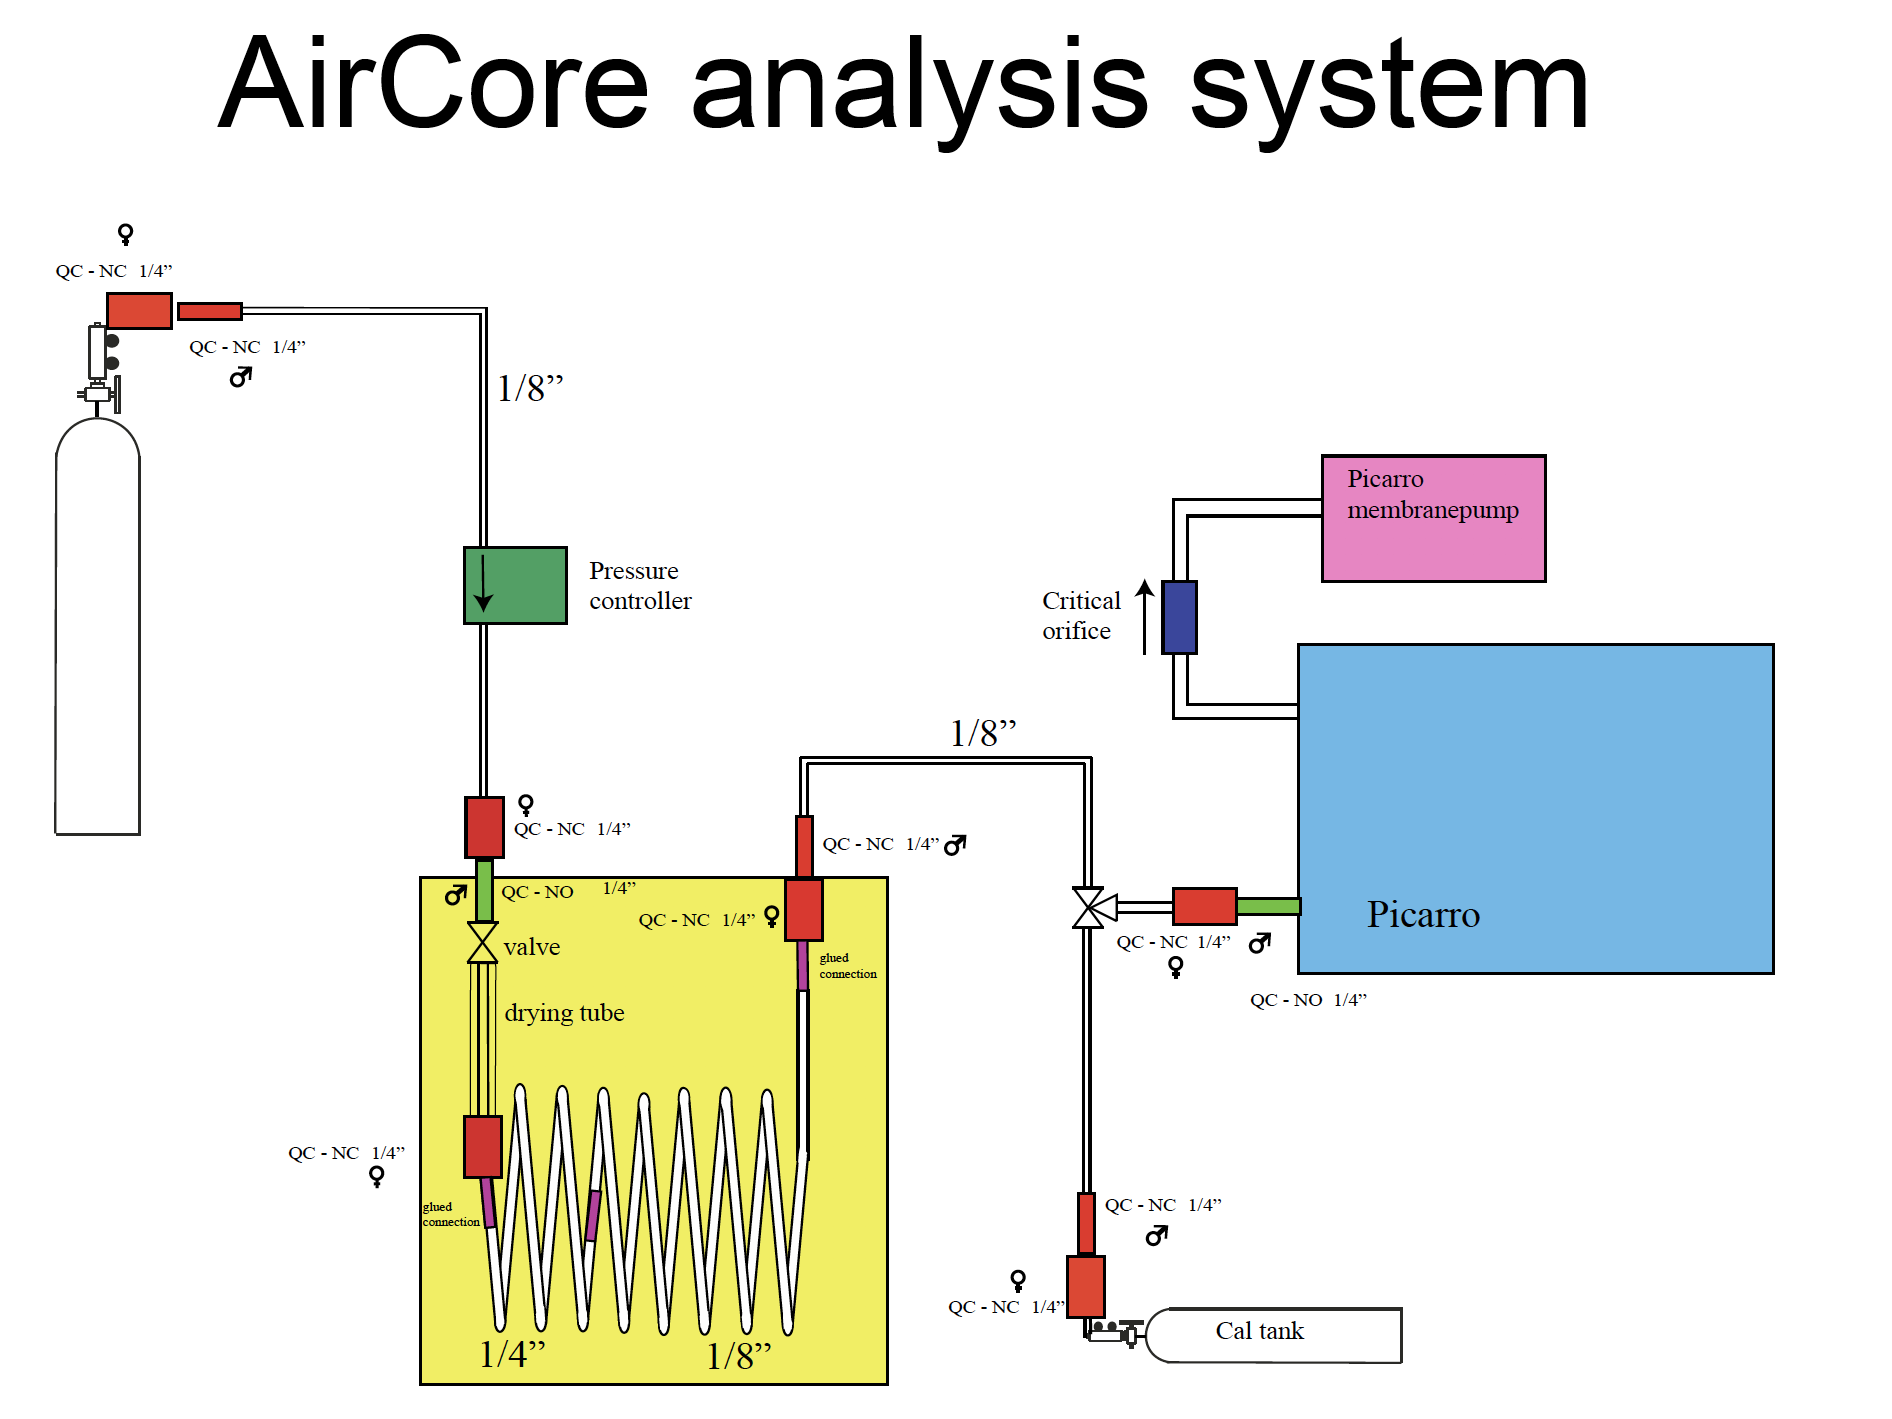
\includegraphics[width=0.9\linewidth]{7-data-analysis-and-results/img/aircore-analysis.png}
    \end{align*}
    \caption{Schematics of CAC Analysis System \cite{AircoreFlights}. \label{fig:aircore-analysis}}
\end{figure}

The analyzer pump and the push gas help the sample to go through the analyzer. The analysis will be started from the side which contains the samples taken at higher altitudes to avoid losing resolution. The beginning and end of the sample analysis is detected due to changes in concentrations, at the beginning between calibrating gas/sample, and at the end, between sample/fill gas. Once the analysis is done, the sample taken with the CAC is stored in a sampler as seen in Figure \ref{fig:aircore-sampler}. This CAC sampler is at FMI and contains fifteen separate sections. All the valves are open when the sample is introduced. Once the analysis is finished and the whole sample is in the sampler, all the valves are closed at the same time, separating the samples for different altitudes and preventing further molecular diffusion.  


\begin{figure}[H]
    \begin{align*}
        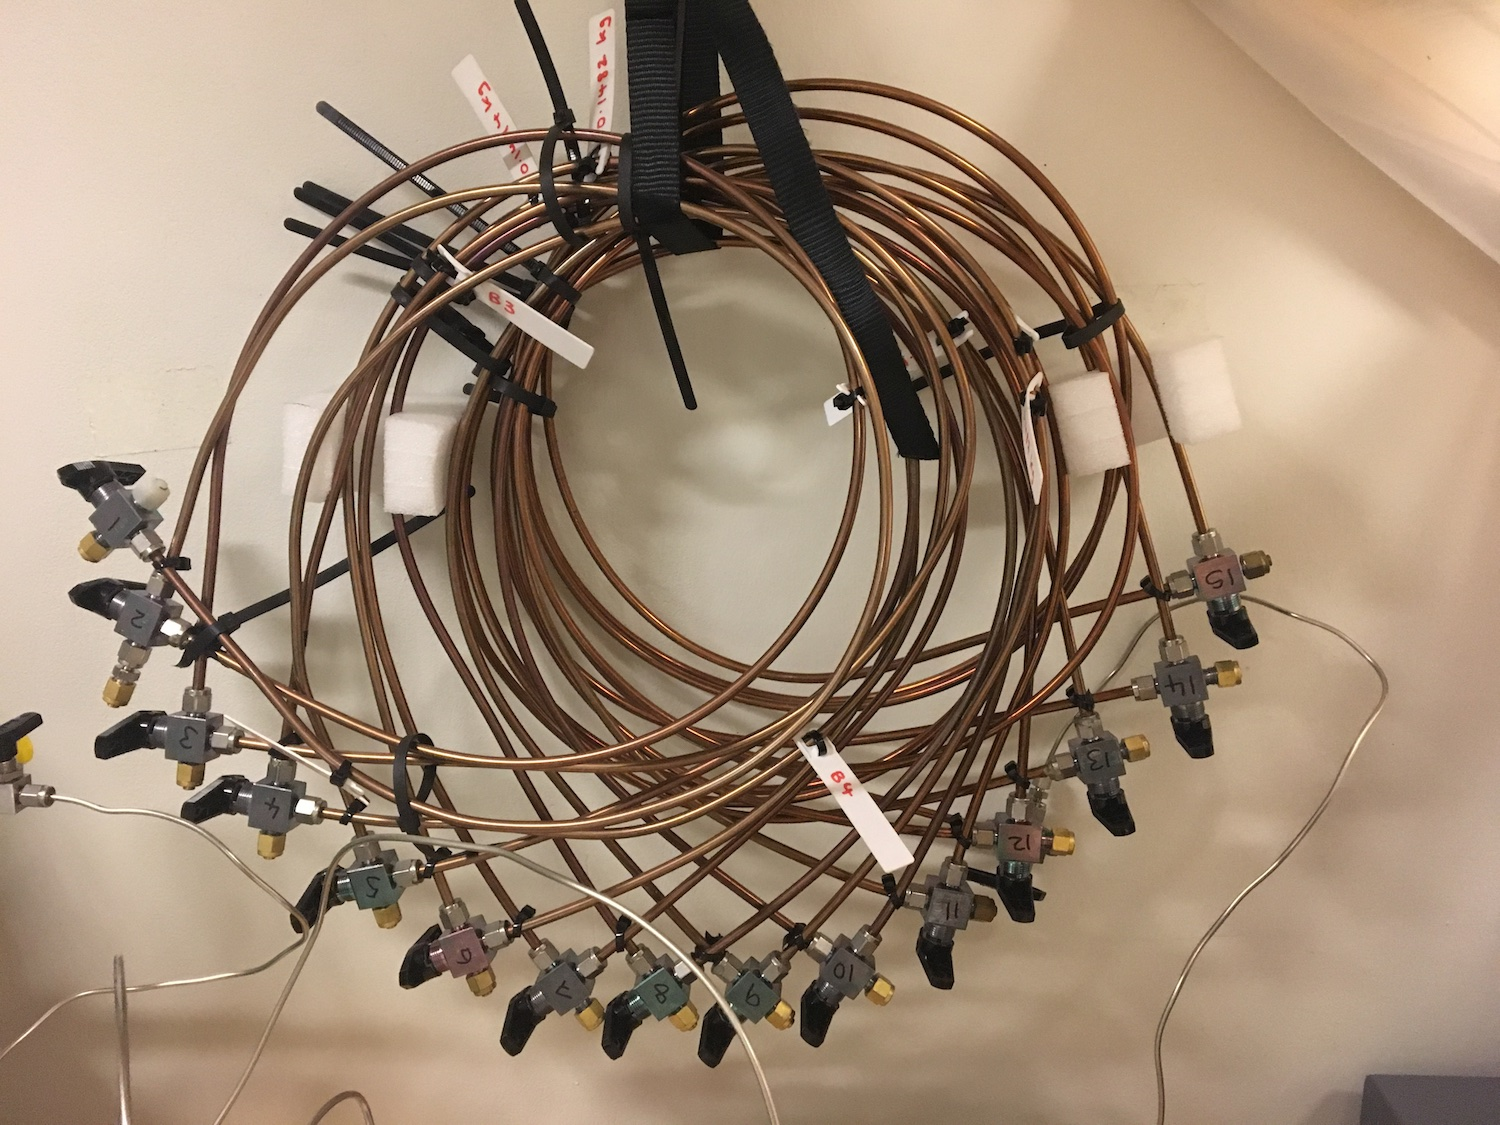
\includegraphics[width=0.9\linewidth]{7-data-analysis-and-results/img/aircore-sampler.jpeg}
    \end{align*}
    \caption{CAC Sampler with 15 Different Stages. \label{fig:aircore-sampler}}
\end{figure}


After the sample has been analyzed, the time trace of analysis will be converted into a mole fraction profile as a function of atmospheric pressure, using the ideal gas law,
\begin{equation}
    PV = nRT <=> n = \frac{PV}{RT}
    \label{eq:idealgaslaw}
\end{equation}
where P is the ambient pressure, V is the inner volume of the CAC/AAC, n the fraction of moles, R is the universal gas constant in $J K^{-1} mol^{-1}$ and T the ambient temperature in Kelvin, \cite{Membrive}. 
A constant unit of pressure in the atmosphere is represented by a unit of length in the CAC tube, due to the method that the CAC will sample the ambient air.

During the analysis the number of moles that will go through the analyzer will increase linearly with time. So, the number of moles at any time during the analysis will be
\begin{equation}
    n_i = n^{max}\frac{t_i}{\Delta t}
    \label{eq:ni}
\end{equation}
where $n^{max}$ is the maximum number of moles i.e when the CAC reaches the Earth's surface, and $\Delta t$ is the total time duration of the analysis between the top and bottom of the CAC sample.   

Finally, the vertical profiles will be obtained by using equations \ref{eq:idealgaslaw} and \ref{eq:ni}, and relate a specific pressure point with every Picarro measurement of the sample.   

The AAC sampling system will be analyzed, in the same manner as the CAC, using the same Picarro gas analyzer. In the same way as for the CAC, the calibrating gas needs to be flowing through the analyzer until the moisture is minimum and the readings in concentrations are stable. Then a sampling bags system will be connected to the analyzer and a dry gas bottle, in a similar way as it was done in Test 17. The tubes connecting the sampling bags will be flushed with dry gas and when the concentrations given by the Picarro analyzer are stable, the air inside the sampling bags will go through the analyzer followed again by dry gas.  

Watching at the Picarro GUI, it is easily recognizable when a sampling bag is being analyzed due to the difference in concentrations between its air and the dry gas. 

Again, as for the CAC, equations \ref{eq:idealgaslaw} and \ref{eq:ni} are going to be used to relate a specific pressure point with every Picarro measurement of the sample. 


The basic working principle used by the chromatographer to obtain the concentrations is as follows:
\begin{itemize}
    \item Have calibrating gas - sample - calibrating gas flowing through the analyzer. (It could also be the case: calibrating gas - dry gas - sample - dry gas - calibrating gas but the principle is the same). 
    \item Identify in the GUI readings the different gases easily seen by sudden variations in the concentrations. 
    \item Compare the calibrating gas reading with the known real value. Do this before and after the sample. This difference corresponds to the drift given by the Picarro. 
    \item Interpolate the values of drift from before and after the sample to obtain the drift during the sample. 
    \item Correct the readings given by the Picarro analyzer due to drift and that is the real concentration value. 
\end{itemize}

NOTE: A calibrating gas is a gas that has been flowing through the Picarro analyzer multiple times and its concentration is known with accuracy. A calibrating gas has to flow before and after the samples in order to compare the readings given by the analyzer with the real value and obtain a corrected value for the samples. 

